\subsection{Design of "Apps" Settings}\label{sprint3:design:apps}

A requirement from Sprint 2 was a pane in settings, where it can be set up which applications each user has access to.
 \lstinline!SettingsActivity! loads fragments into its container, but because "Apps" should distinguish between \giraf and other Android applications, an additional fragmentcontainer needs to be inserted.
 The idea can be seen visualized in \cref{fig:settingsappfragments}.
 
\begin{figure}[h]
\centering
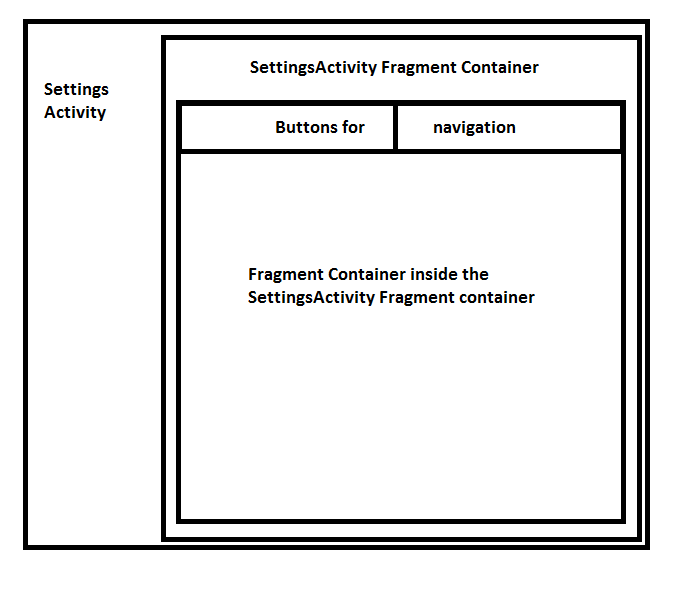
\includegraphics[width=\textwidth, height=3in, keepaspectratio=true] {SettingsActivity.png}
\caption{The organization of \lstinline!SettingsActivity! when inside the "Apps" pane. Since we need to distinguish between \giraf and Android applications, nested fragment containers are used.}
\label{fig:settingsappfragments}
\end{figure}

Because the \giraf and Android pane fragments will contain many of the same variables, these should inherit all shared information from a superclass, consequently reducing redundancy and clarifying how the two fragments are different.

Finally, the navigation buttons inside the \lstinline!SettingsActivity! fragment container should also have a button opening the Google Play Store, so the user can download additional Android applications, if desired. 